\noindent ChatGPT and the realm of search engine AI's were particularly useful in this research process for identifying the different types of technologies currently available, given the market observable on the internet. However, the LLM tended to struggle with providing accurate and specifications from datasheets, requiring the researchers to sift through and locate them. Additionally, ChatGPT was useful for preparing references for sources, but even in this it sometimes struggled to gather the correct article or paper title, although it was strong in being able to provide them in most formats including the IEEE reference style.\\

\subsection{Example 1: Sonar vs. LiDAR}
\noindent One specific example of ChatGPT aiding the research process is by providing a concise explanation of the comparison between the Sonar and LiDAR sensing methods. It is able to be objective and pull from all knowledge of these technologies to best inform our decisions.\\
\begin{figure}[H]
	\centering
	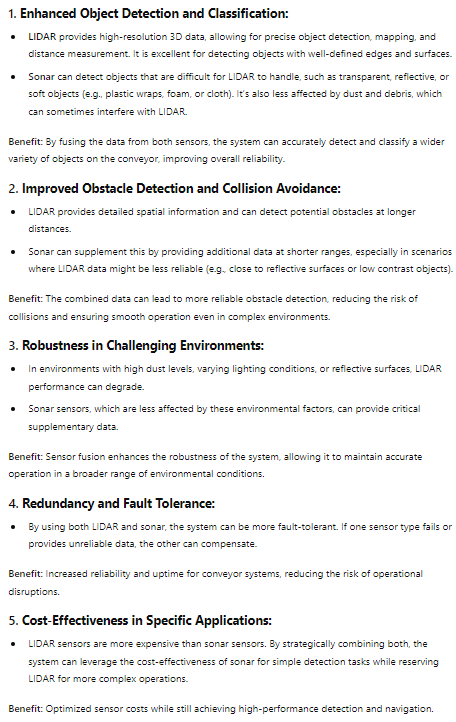
\includegraphics[width=0.5\textwidth]{./Images/chatgpt1.png}
	\caption{\label{fig:chatgpt1}ChatGPT compares sensing technologies}
\end{figure}

% NEED TO CITE CHATGPT

\subsection{Example 2: Power Supply to the MCU}
\noindent ChatGPT proved to be very useful for the sake of research, particularly when there were specific concerns. In this example, we used ChatGPT to answer a question of compatibility in order to determine how many power sources were necessary to purchase. The response both clearly and concisely answered the question with several conditions to keep in mind. Thus, one of the main advantages to generative AI is that it provides a direct answer to a specific question, automatically sifting through information that is irrelevant. Very often, a simple Google search will draw only a certain sentence or paragraph from a website that relates to the query, while the rest of the website may or may not be relevant. ChatGPT instead combines several sources with almost all relevant information so that less investigating is required. However, one advantage to a Google search is that you are able to see the source of the answer and understand the surrounding context. For example, you may create a query asking how a motor driver works, meanwhile you do not know how DC motors work in general. A Google search may provide a website that provides preliminary information on the functionality of DC motors before diving into the functionality of motor drivers themselves. On the contrary, ChatGPT only would have provided information on motor drivers themselves. This is advantageous when you are unsure where to start researching or "don't know what you don't know."

\noindent Prompt: Can you power microcontroller and motors with the same battery pack?\\

\noindent Response from ChatGPT:\\

\noindent Yes, you can power a microcontroller and motors with the same battery pack, but there are a few considerations to keep in mind:\\

\noindent Voltage Compatibility: Ensure that the battery pack provides a voltage compatible with both the microcontroller and the motors. For example, if the microcontroller operates at 5V and the motors require 6V, you'll need a way to regulate the voltage for the microcontroller.\\

\noindent Current Requirements: Motors can draw significantly more current than microcontrollers. Make sure the battery pack can supply enough current for both without causing voltage drops that might reset the microcontroller.\\

\noindent Noise and Interference: Motors can introduce electrical noise, especially when they start or change speed. It’s a good idea to use decoupling capacitors near the microcontroller and possibly include a separate power supply or filtering for sensitive components.\\

\noindent Power Management: If the microcontroller is in sleep mode or only occasionally active, consider using a power management system to optimize battery life.\\

\noindent Common Ground: Make sure that both the microcontroller and motors share a common ground to avoid potential issues with signal integrity.\\

\noindent By keeping these factors in mind, you can successfully power both components from the same battery pack!
\subsection{Example 3: }